% Source: graduate-coursework/Prior_Semesters/Fa25/EMCH501/HW4/HW4.tex

\documentclass[border=4pt]{standalone}
\usepackage{amsmath}
\usepackage{amssymb}
\usepackage{graphicx}
\usepackage{pgfplots}
\usepackage{tikz}
\usepackage{xcolor}
\pgfplotsset{compat=1.18}
\usetikzlibrary{shapes.geometric, arrows.meta, positioning, decorations.pathmorphing, patterns}

\definecolor{USC_Garnet}{HTML}{73000A}
\definecolor{USC_Sandstorm}{HTML}{FFF2E3}
\definecolor{USC_Black90}{HTML}{565656}
\definecolor{USC_Black10}{HTML}{ECECEC}
\definecolor{USC_Honeycomb}{HTML}{65780B}
\definecolor{tablegreen}{RGB}{230,242,230}
\definecolor{outputbg}{RGB}{245,245,245}


\begin{document}
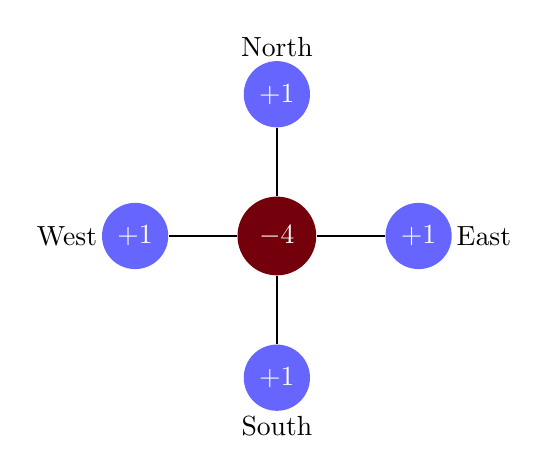
\begin{tikzpicture}[scale=1.2]
    % Center node
    \node[circle, fill=USC_Garnet, text=white, minimum size=1cm] (C) at (0,0) {$-4$};
    % Neighbor nodes
    \node[circle, fill=blue!60, text=white, minimum size=0.8cm] (E) at (1.5,0) {$+1$};
    \node[circle, fill=blue!60, text=white, minimum size=0.8cm] (W) at (-1.5,0) {$+1$};
    \node[circle, fill=blue!60, text=white, minimum size=0.8cm] (N) at (0,1.5) {$+1$};
    \node[circle, fill=blue!60, text=white, minimum size=0.8cm] (S) at (0,-1.5) {$+1$};
    % Lines
    \draw[thick] (C) -- (E); \draw[thick] (C) -- (W);
    \draw[thick] (C) -- (N); \draw[thick] (C) -- (S);
    % Labels
    \node[right] at (1.8,0) {East};
    \node[left] at (-1.8,0) {West};
    \node[above] at (0,1.8) {North};
    \node[below] at (0,-1.8) {South};
\end{tikzpicture}
\end{document}
